\chapter{Desenvolvimento do Sistema}

\section{Visão Geral do Projeto}

A aplicação desenvolvida tem como objetivo principal automatizar a quantificação do crescimento de plantas a partir de imagens digitais, proporcionando uma ferramenta acessível para pesquisadores, agrônomos e demais interessados. Por meio do processamento automatizado de fotos, o sistema permite extrair medidas morfológicas relevantes (área, altura e largura) de plantas ao longo do tempo, facilitando o acompanhamento do desenvolvimento vegetal em experimentos ou cultivos. A interface gráfica foi projetada para tornar o processo intuitivo, desde a organização das imagens em coleções até a visualização dos resultados e geração de gráficos de crescimento, promovendo eficiência na análise de dados.

\begin{figure}[H]
    \centering
    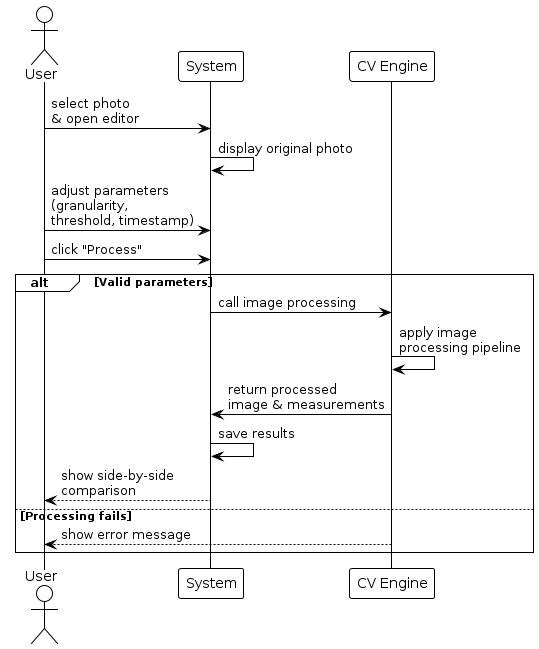
\includegraphics[width=0.45\textwidth]{../figures/dss/UC011.png}
    \caption{Diagrama de sequência do processamento de uma foto individual. Fonte: os autores}
    \label{fig:uc011-process-single-photo}
\end{figure}

\subsection{Processamento de Imagem}

A quantificação do crescimento de plantas a partir de imagens envolve uma série de conceitos fundamentais de processamento de imagem, com destaque para segmentação, análise de cor e extração de medidas morfológicas. O primeiro desafio é separar a planta do fundo da imagem, tarefa conhecida como segmentação.

Para isso, utilizamos o algoritmo watershed. O algoritmo interpreta a imagem em tons de cinza como uma superfície topográfica, onde os valores de intensidade representam elevações. Inicialmente, marcadores são definidos em regiões de interesse (como fundo e possíveis objetos). A partir desses marcadores, o algoritmo simula o preenchimento dessas regiões com "água". À medida que a água se espalha, ela encontra barreiras naturais (bordas) e, quando duas regiões em expansão se encontram, uma linha de separação é criada, formando as fronteiras entre os objetos segmentados. Esse processo resulta em uma segmentação precisa, especialmente útil para separar objetos conectados ou com contornos pouco definidos.

Após a segmentação, é necessário identificar qual das regiões corresponde de fato à planta. Para isso, analisamos as propriedades de cor das regiões segmentadas, utilizando tanto o modelo tradicional RGB (ou BGR) quanto o modelo HSV, que separa matiz, saturação e valor. A predominância de tons de verde é o principal critério para reconhecer a área foliar, já que a maioria das plantas apresenta essa característica. O uso combinado de diferentes espaços de cor torna o processo mais robusto a variações de iluminação e tonalidade.

Com a planta isolada, aplicam-se operações morfológicas para corrigir pequenas falhas na máscara, como buracos ou regiões desconectadas, garantindo que a área da planta seja representada de forma contínua. A partir dessa máscara, extraímos medidas morfológicas relevantes: a área, dada pela contagem de pixels; a altura, que corresponde à maior extensão da planta ao longo de seu eixo principal, obtida por regressão linear dos pontos segmentados; e a largura, medida perpendicularmente à altura. Essas medidas permitem acompanhar o desenvolvimento da planta ao longo do tempo de maneira objetiva e automatizada.

Por fim, a visualização dos resultados é facilitada pela sobreposição da máscara segmentada e das linhas de medição sobre a imagem original, tornando o processo interpretável e útil para o usuário.

\subsection{Interface Gráfica}

A interface gráfica da aplicação oferece um conjunto de funcionalidades que tornam o acompanhamento do crescimento de plantas prático e eficiente. O usuário pode criar coleções para organizar fotos de uma mesma planta ou experimento ao longo do tempo, facilitando o gerenciamento e a comparação dos resultados. É possível associar ou desassociar fotos de uma coleção, renomear ou excluir coleções inteiras, e visualizar todas as imagens agrupadas de forma estruturada.

Além disso, a interface permite o envio e processamento de fotos individuais ou múltiplas de uma só vez, tornando simples tanto testes rápidos quanto o acompanhamento de experimentos. Após o processamento, o usuário pode visualizar as imagens segmentadas com as medidas extraídas (área, altura e largura) e acessar detalhes de cada foto, incluindo os resultados obtidos.

Outro recurso importante é a geração automática de gráficos de crescimento para cada coleção, permitindo ao usuário acompanhar visualmente a evolução das plantas ao longo do tempo.

\section{Implementação}

\subsection{Segmentação da Imagem}

A detecção e quantificação da planta na imagem é realizada por meio de um pipeline de processamento implementado no arquivo \texttt{processImage.py}. O funcionamento do algoritmo pode ser descrito nas seguintes etapas principais:

\subsubsection{Leitura e validação da entrada}
Para o recebimento das informações necessárias ao processamento, o sistema utiliza um identificador único para cada imagem processada. Esse identificador é utilizado para localizar um arquivo JSON correspondente, que contém os parâmetros de granularidade e limiar de separação, juntamente com a imagem a ser analisada (codificada em base64).

Essa abordagem foi adotada devido à flexibilidade do formato JSON, que facilita a integração com diferentes sistemas e interfaces. Além disso, o sistema realiza a validação da versão do Python e das dependências, assegurando a compatibilidade do ambiente de execução e prevenindo falhas de difícil diagnóstico.

\subsubsection{Decodificação e pré-processamento}
Após a leitura dos dados, a imagem é decodificada do formato base64. Caso necessário, ela é redimensionada para que o maior lado não ultrapasse 1024 pixels. O redimensionamento adaptativo busca equilibrar a preservação de detalhes relevantes com a eficiência computacional, tornando o sistema apto a lidar com imagens de diferentes origens e qualidades.

O pré-processamento inclui a conversão para tons de cinza (requisito do watershed) aplicação de desfoque gaussiano adaptativo e realce de contraste local com CLAHE (Contrast Limited Adaptive Histogram Equalization). Essas técnicas reduzem ruídos, pequenas variações locais e aumentam a distinção entre planta e fundo, especialmente em condições de iluminação heterogênea.

\subsubsection{Detecção de bordas e segmentação}
A detecção de bordas é realizada com o filtro de Sobel, seguida de fechamento morfológico para eliminar pequenas falhas e descontinuidades nas bordas. Essas operações preparam a imagem para a segmentação, que é realizada pelo algoritmo watershed.

O watershed foi escolhido por sua robustez na separação de regiões conectadas em imagens complexas, simulando o "alastramento" de água a partir de marcadores. Os marcadores são distribuídos de forma adaptativa conforme o tamanho da imagem e o parâmetro de granularidade, conferindo maior generalidade e precisão ao método.

\subsubsection{Identificação da região da planta}
Após a segmentação, cada região é analisada em dois espaços de cor (BGR e HSV) para identificar aquelas com predominância de verde, correspondentes à planta.

O uso combinado desses espaços de cor, aliado a critérios adaptativos e thresholds ajustáveis, torna a identificação robusta a diferentes condições de iluminação, tonalidade e espécies vegetais, mitigando falsos positivos em regiões esmaecidas ou sombreadas.

\subsubsection{Pós-processamento da máscara}
A máscara resultante da segmentação pode apresentar buracos ou falhas devido a reflexos, sombras ou limitações do processo segmentativo. Para garantir a continuidade da área foliar, são aplicadas operações morfológicas de fechamento e preenchimento de buracos.

O tamanho mínimo dos buracos a serem preenchidos é ajustado dinamicamente conforme o tamanho da imagem. Essa etapa é fundamental para a extração acurada das medidas morfológicas.

\subsubsection{Extração de medidas}
Com a máscara da planta definida, o sistema extrai os pixels correspondentes e calcula as principais medidas morfológicas: altura (por regressão linear dos pontos segmentados), largura (projeção no eixo perpendicular à reta ajustada) e área (contagem de pixels segmentados).

A escolha da regressão linear permite a obtenção da extensão máxima da planta ao longo do eixo principal, independentemente da orientação da imagem.

\subsubsection{Geração da imagem de saída}
Por fim, a imagem original recebe uma sobreposição da máscara segmentada e das linhas de medição (altura em amarelo, largura em magenta), com marcadores circulares nas extremidades para destacar os pontos de referência. O resultado é codificado em base64 (JPEG ou PNG).

\vspace{1.5cm}

O conjunto dessas etapas resulta em um pipeline flexível, robusto e eficiente, capaz de lidar com diferentes condições de imagem e cenários experimentais.

\subsection{Interface Gráfica}

A interface gráfica da aplicação foi desenvolvida utilizando Electron, uma plataforma que permite criar aplicações desktop multiplataforma com tecnologias web (HTML, CSS e JavaScript). O uso do Electron possibilita que a interface seja executada de forma nativa em diferentes sistemas operacionais, mantendo uma experiência consistente para o usuário. O Electron também foi escolhido por não depender de servidores externos, garantindo maior privacidade.

A comunicação entre a interface e o backend de processamento de imagens é feita de forma transparente, permitindo que o usuário acompanhe o status das operações e visualize rapidamente os resultados.

Dessa forma, a aplicação proporciona uma solução completa e acessível para o acompanhamento automatizado do crescimento de plantas, aliando facilidade de uso, portabilidade e integração eficiente entre interface e processamento de dados.

\section{Dificuldades}

Durante o desenvolvimento do projeto, uma das principais dificuldades encontradas foi a detecção dos caules das plantas nas imagens. Apesar de diversos esforços, não foi possível obter resultados minimamente satisfatórios para a identificação automática dessa estrutura, ao contrário do que foi alcançado para as folhas.

Inicialmente, tentamos aplicar uma abordagem semelhante à utilizada para as folhas, buscando separar os caules pela cor marrom, utilizando limiares nos espaços de cor BGR e HSV. No entanto, a grande variação de tonalidade dos caules — que podem variar do marrom claro ao quase esverdeado ou acinzentado — dificultou a definição de um intervalo de cor robusto. Além disso, a presença de sombras projetadas pelas próprias folhas, reflexos do solo úmido e a semelhança de cor dos caules com o substrato e galhos secos frequentemente resultaram em uma segmentação com muitos falsos positivos e negativos.

Tentamos também técnicas baseadas em morfologia e geometria, como a aplicação da transformada de Radon, que pode ser útil para detectar estruturas lineares verticais, típicas de caules. No entanto, nas imagens reais, os caules frequentemente não aparecem como linhas contínuas devido à sobreposição de folhas, curvaturas naturais, variações de espessura e interrupções causadas por outros elementos da planta ou do fundo. Isso fez com que a resposta da transformada de Radon fosse difusa e pouco informativa, sem permitir a extração de segmentos confiáveis.

Por fim, exploramos o uso de métodos de aprendizado de máquina, incluindo tentativas com classificadores tradicionais e redes neurais convolucionais. No entanto, a ausência de um conjunto de dados anotado especificamente para caules, aliado à grande variabilidade visual dessa estrutura entre diferentes espécies e estágios de desenvolvimento, dificultou o treinamento de modelos generalizáveis. Os resultados obtidos apresentaram baixa precisão e alta taxa de erro, especialmente em imagens com fundo complexo ou iluminação não controlada.

\begin{figure}[H]
    \centering
    % Imagens dos resultados das tentativas de ML para detecção de caules
    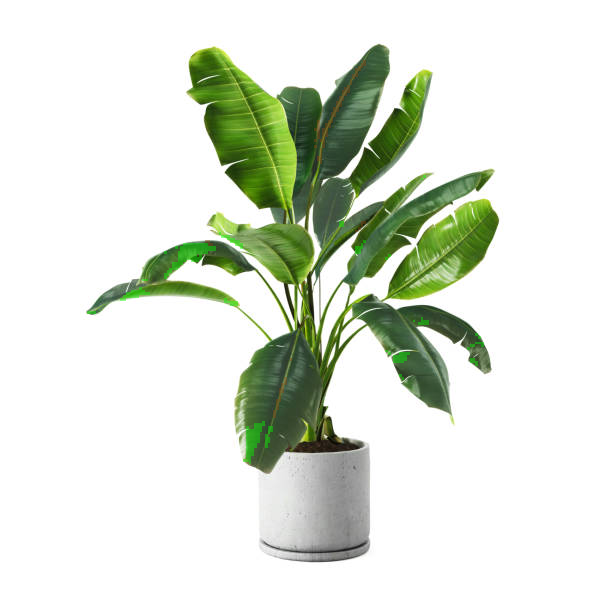
\includegraphics[height=4cm]{../figures/ml_results/attempt1.png}
    \hspace{0.2cm}
    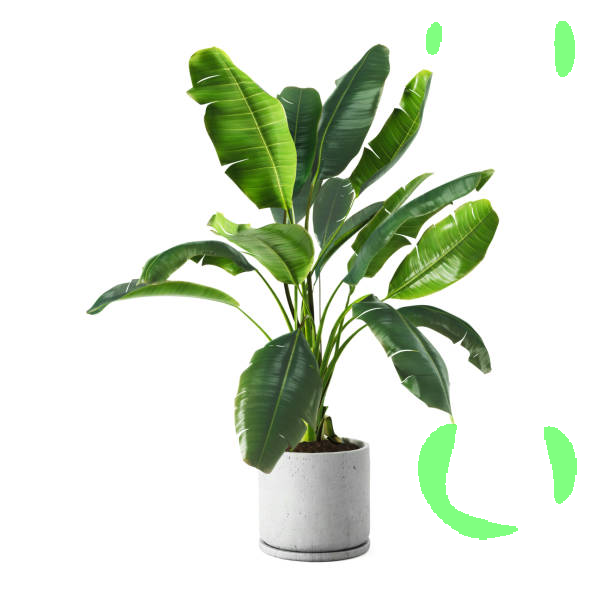
\includegraphics[height=4cm]{../figures/ml_results/attempt2.png}
    \hspace{0.2cm}
    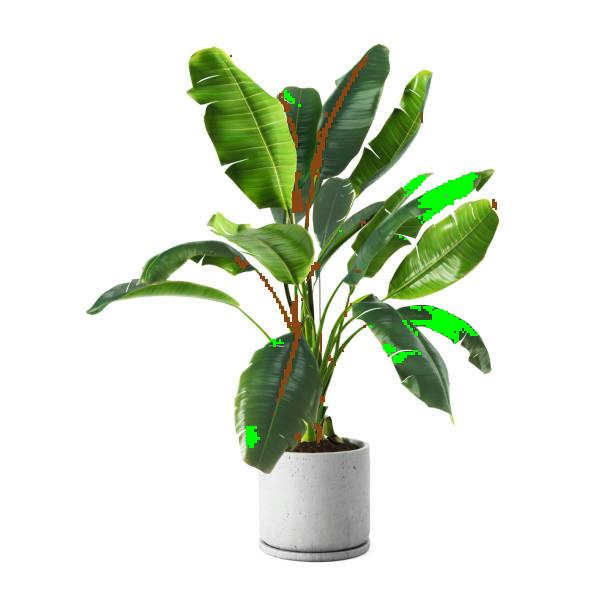
\includegraphics[height=4cm]{../figures/ml_results/attempt3.jpg}
    \caption{Exemplos de tentativas frustradas de detecção automática de caules utilizando diferentes abordagens de machine learning. Fonte: os autores.}
    \label{fig:ml_failed_attempts}
\end{figure}

Dessa forma, a solução final do projeto ficou restrita à detecção e quantificação das folhas, que apresentaram características visuais mais homogêneas e segmentáveis nas imagens disponíveis, permitindo resultados mais confiáveis e reprodutíveis.
